\documentclass{standalone}

\usepackage{pgfplots,tikz,amsmath}
\begin{document}
    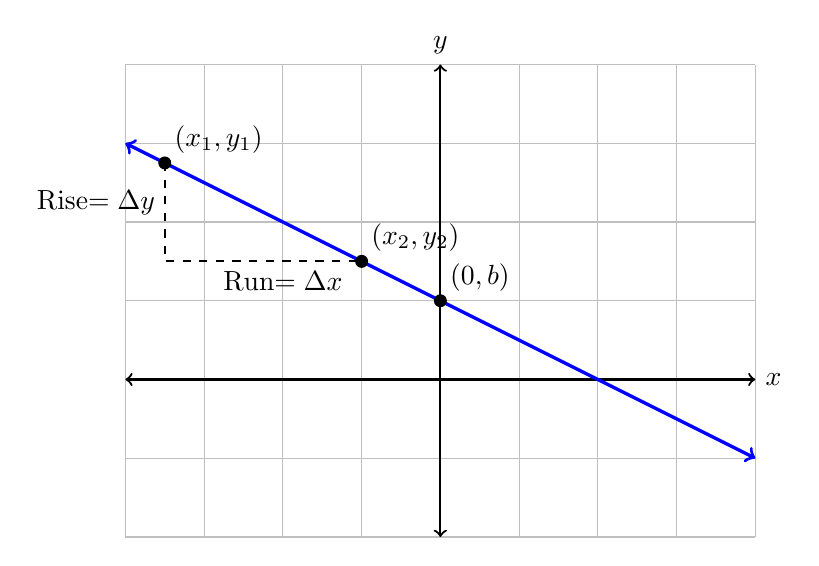
\begin{tikzpicture}
        \draw[color=gray!50] (-4,-2) grid (4,4);
        \draw[<->, thick] (-4,0) -- (4,0) node[anchor=west]{$x$};
        \draw[<->, thick] (0,-2) -- (0,4) node[anchor=south]{$y$};
        \draw[<->, very thick, blue] (-4,3) -- (4,-1);
        \draw[color=black, fill=black] (-3.5,2.75) circle(0.075cm) node[anchor=south
        west]{$(x_1,y_1)$};
        \draw[color=black, fill=black] (-1,1.5) circle(0.075cm) node[anchor=south
        west]{$(x_2,y_2)$};
        \draw[color=black, fill=black] (0,1) circle(0.075cm) node[anchor=south
        west]{$(0,b)$};
        \draw[thick, dashed] (-3.5,2.75) -- (-3.5,1.5) -- (-1,1.5);
        \draw (-3.5,2.25) node[anchor=east]{Rise$=\Delta y$};
        \draw (-2,1.5) node[anchor=north]{Run$=\Delta x$};
    \end{tikzpicture}
\end{document}
